%File: report.tex
\documentclass[letterpaper]{article} % DO NOT CHANGE THIS
\usepackage{aaai25}  % DO NOT CHANGE THIS
\usepackage{times}  % DO NOT CHANGE THIS
\usepackage{helvet}  % DO NOT CHANGE THIS
\usepackage{courier}  % DO NOT CHANGE THIS
\usepackage[hyphens]{url}  % DO NOT CHANGE THIS
\usepackage{graphicx} % DO NOT CHANGE THIS
\urlstyle{rm} % DO NOT CHANGE THIS
\def\UrlFont{\rm}  % DO NOT CHANGE THIS
\usepackage{natbib}  % DO NOT CHANGE THIS AND DO NOT ADD ANY OPTIONS TO IT
\usepackage{caption} % DO NOT CHANGE THIS AND DO NOT ADD ANY OPTIONS TO IT
\frenchspacing  % DO NOT CHANGE THIS
\setlength{\pdfpagewidth}{8.5in} % DO NOT CHANGE THIS
\setlength{\pdfpageheight}{11in} % DO NOT CHANGE THIS
%
% These are recommended to typeset algorithms but not required. See the subsubsection on algorithms. Remove them if you don't have algorithms in your paper.
\usepackage{algorithm}
\usepackage{algorithmic}

%
% These are are recommended to typeset listings but not required. See the subsubsection on listing. Remove this block if you don't have listings in your paper.
\usepackage{newfloat}
\usepackage{listings}
\DeclareCaptionStyle{ruled}{labelfont=normalfont,labelsep=colon,strut=off} % DO NOT CHANGE THIS
\lstset{%
	basicstyle={\footnotesize\ttfamily},% footnotesize acceptable for monospace
	numbers=left,numberstyle=\footnotesize,xleftmargin=2em,% show line numbers, remove this entire line if you don't want the numbers.
	aboveskip=0pt,belowskip=0pt,%
	showstringspaces=false,tabsize=2,breaklines=true}
\floatstyle{ruled}
\newfloat{listing}{tb}{lst}{}
\floatname{listing}{Listing}
%
% Keep the \pdfinfo as shown here. There's no need
% for you to add the /Title and /Author tags.
\pdfinfo{
/TemplateVersion (2025.1)
}

% DISALLOWED PACKAGES
% \usepackage{authblk} -- This package is specifically forbidden
% \usepackage{balance} -- This package is specifically forbidden
% \usepackage{color (if used in text)
% \usepackage{CJK} -- This package is specifically forbidden
% \usepackage{float} -- This package is specifically forbidden
% \usepackage{flushend} -- This package is specifically forbidden
% \usepackage{fontenc} -- This package is specifically forbidden
% \usepackage{fullpage} -- This package is specifically forbidden
% \usepackage{geometry} -- This package is specifically forbidden
% \usepackage{grffile} -- This package is specifically forbidden
% \usepackage{hyperref} -- This package is specifically forbidden
% \usepackage{navigator} -- This package is specifically forbidden
% (or any other package that embeds links such as navigator or hyperref)
% \indentfirst} -- This package is specifically forbidden
% \layout} -- This package is specifically forbidden
% \multicol} -- This package is specifically forbidden
% \nameref} -- This package is specifically forbidden
% \usepackage{savetrees} -- This package is specifically forbidden
% \usepackage{setspace} -- This package is specifically forbidden
% \usepackage{stfloats} -- This package is specifically forbidden
% \usepackage{tabu} -- This package is specifically forbidden
% \usepackage{titlesec} -- This package is specifically forbidden
% \usepackage{tocbibind} -- This package is specifically forbidden
% \usepackage{ulem} -- This package is specifically forbidden
% \usepackage{wrapfig} -- This package is specifically forbidden
% DISALLOWED COMMANDS
% \nocopyright -- Your paper will not be published if you use this command
% \addtolength -- This command may not be used
% \balance -- This command may not be used
% \baselinestretch -- Your paper will not be published if you use this command
% \clearpage -- No page breaks of any kind may be used for the final version of your paper
% \columnsep -- This command may not be used
% \newpage -- No page breaks of any kind may be used for the final version of your paper
% \pagebreak -- No page breaks of any kind may be used for the final version of your paperr
% \pagestyle -- This command may not be used
% \tiny -- This is not an acceptable font size.
% \vspace{- -- No negative value may be used in proximity of a caption, figure, table, section, subsection, subsubsection, or reference
% \vskip{- -- No negative value may be used to alter spacing above or below a caption, figure, table, section, subsection, subsubsection, or reference

\setcounter{secnumdepth}{2} %May be changed to 1 or 2 if section numbers are desired.

% The file aaai25.sty is the style file for AAAI Press
% proceedings, working notes, and technical reports.
%

\usepackage{amsmath}
\usepackage{hyperref}
\hypersetup{
    colorlinks = true,
    allcolors = blue
}

% Title

% Your title must be in mixed case, not sentence case.
% That means all verbs (including short verbs like be, is, using, and go),
% nouns, adverbs, adjectives should be capitalized, including both words in hyphenated terms, while
% articles, conjunctions, and prepositions are lower case unless they
% directly follow a colon or long dash
\title{CS 598 Deep Learning for Healthcare (Spring, 2025)\\Project Report}
\author {Eric Schrock}
\affiliations{ejs9@illinois.edu}

\begin{document}

\maketitle

\begin{abstract}
This report details the results of my final project for CS 598: Deep Learning for Healthcare. My final project had three components.

First, I attempted to reproduce a portion of the findings of the paper "Multi-Label Generalized Zero Shot Learning for the Classification of Disease in Chest Radiographs" \cite{hayat2021multilabel}, specifically the AUROC scores of the proposed model on each of the fourteen diseases labeled in the the dataset. I tried three approaches. The first used the code and pre-trained weights provided by the paper, the second used the provided code but not the provided weights, and the third used neither. Only the first attempt successfully reproduced the AUROC scores reported in the original paper.

Second, I replaced the visual encoder used by the proposed model, DenseNet-121 \cite{huang2018denselyconnectedconvolutionalnetworks}, with the lighter weight EfficientNet-B0 \cite{tan2020efficientnetrethinkingmodelscaling} to see if I could achieve faster training times with comparable AUROC scores. Training was significantly faster, but the AUROC scores were significantly worse.

Third, I submitted a pull request (PR) to PyHealth \cite{pyhealth2023yang}, an open source project dedicated to supporting healthcare-related AI research and applications. My PR added support for the ChestX-ray14 \cite{Wang_2017} dataset and for binary classification tasks on the fourteen diseases labeled in the dataset.

\begin{itemize}
    \item \href{https://drive.google.com/file/d/1fTt2B8VNEQrtBT_Iooby2_viOujf59bX}{Video presentation} \footnote{\url{https://drive.google.com/file/d/1fTt2B8VNEQrtBT_Iooby2_viOujf59bX}}
    \item \href{https://github.com/EricSchrock/cxr-ml-gzsl}{Project GitHub repository} \footnote{\url{https://github.com/EricSchrock/cxr-ml-gzsl}}
    \item \href{https://github.com/sunlabuiuc/PyHealth/pull/392}{PyHealth pull request} \footnote{\url{https://github.com/sunlabuiuc/PyHealth/pull/392}}
\end{itemize}
\end{abstract}

\section{Introduction}

\subsection{Summary of the Paper in Question}

Deep learning models for classifying diseases from chest X-ray (CXR) images have had great success, achieving comparable results to human experts. However, collecting and labeling training data for these models is expensive and time-consuming. For rarer diseases, it is often not economical, and sometimes not even possible, to gather the amount of data needed for supervised learning models. When a new disease emerges, the need for massive data collection slows the response. Human radiologists leverage other sources of knowledge to identify diseases they have previously never seen in X-ray form. Could a deep learning model do the same?

Multi-label generalized zero shot learning (ML-GZSL), which uses semantic information to identify classes not present in the set of labeled images used to train the model, has worked well in similar circumstances \cite{10.1109/TPAMI.2012.256, 10.1109/TMM.2019.2924511, 9157745}. However, these prior works have at least two limitations. First, they "extract a fixed visual representation of the image from a pre-trained visual encoder or a detection network" \cite{hayat2021multilabel}, which means they cannot be trained end-to-end. Second, "projecting these extracted visual features to the semantic space shrinks the diversity of the visual information, which gives rise to inherent limitations" \cite{hayat2021multilabel}, one of those being the hubness problem \cite{dinu2015improvingzeroshotlearningmitigating}. Can these limitations be overcome?

"Multi-Label Generalized Zero Shot Learning for the Classification of Disease in Chest Radiographs" \cite{hayat2021multilabel} proposes the CXR-ML-GZSL model (Figure~\ref{fig:model}). It is comprised of a pre-trained text encoder to convert class labels to a semantic embedding space, a trainable visual encoder to convert X-ray images to a visual embedding space, and mapping models into a shared latent embedding space. The output is a score for each possible class, representing how relevant it is to the input image.

\begin{figure}[h!]
\centering
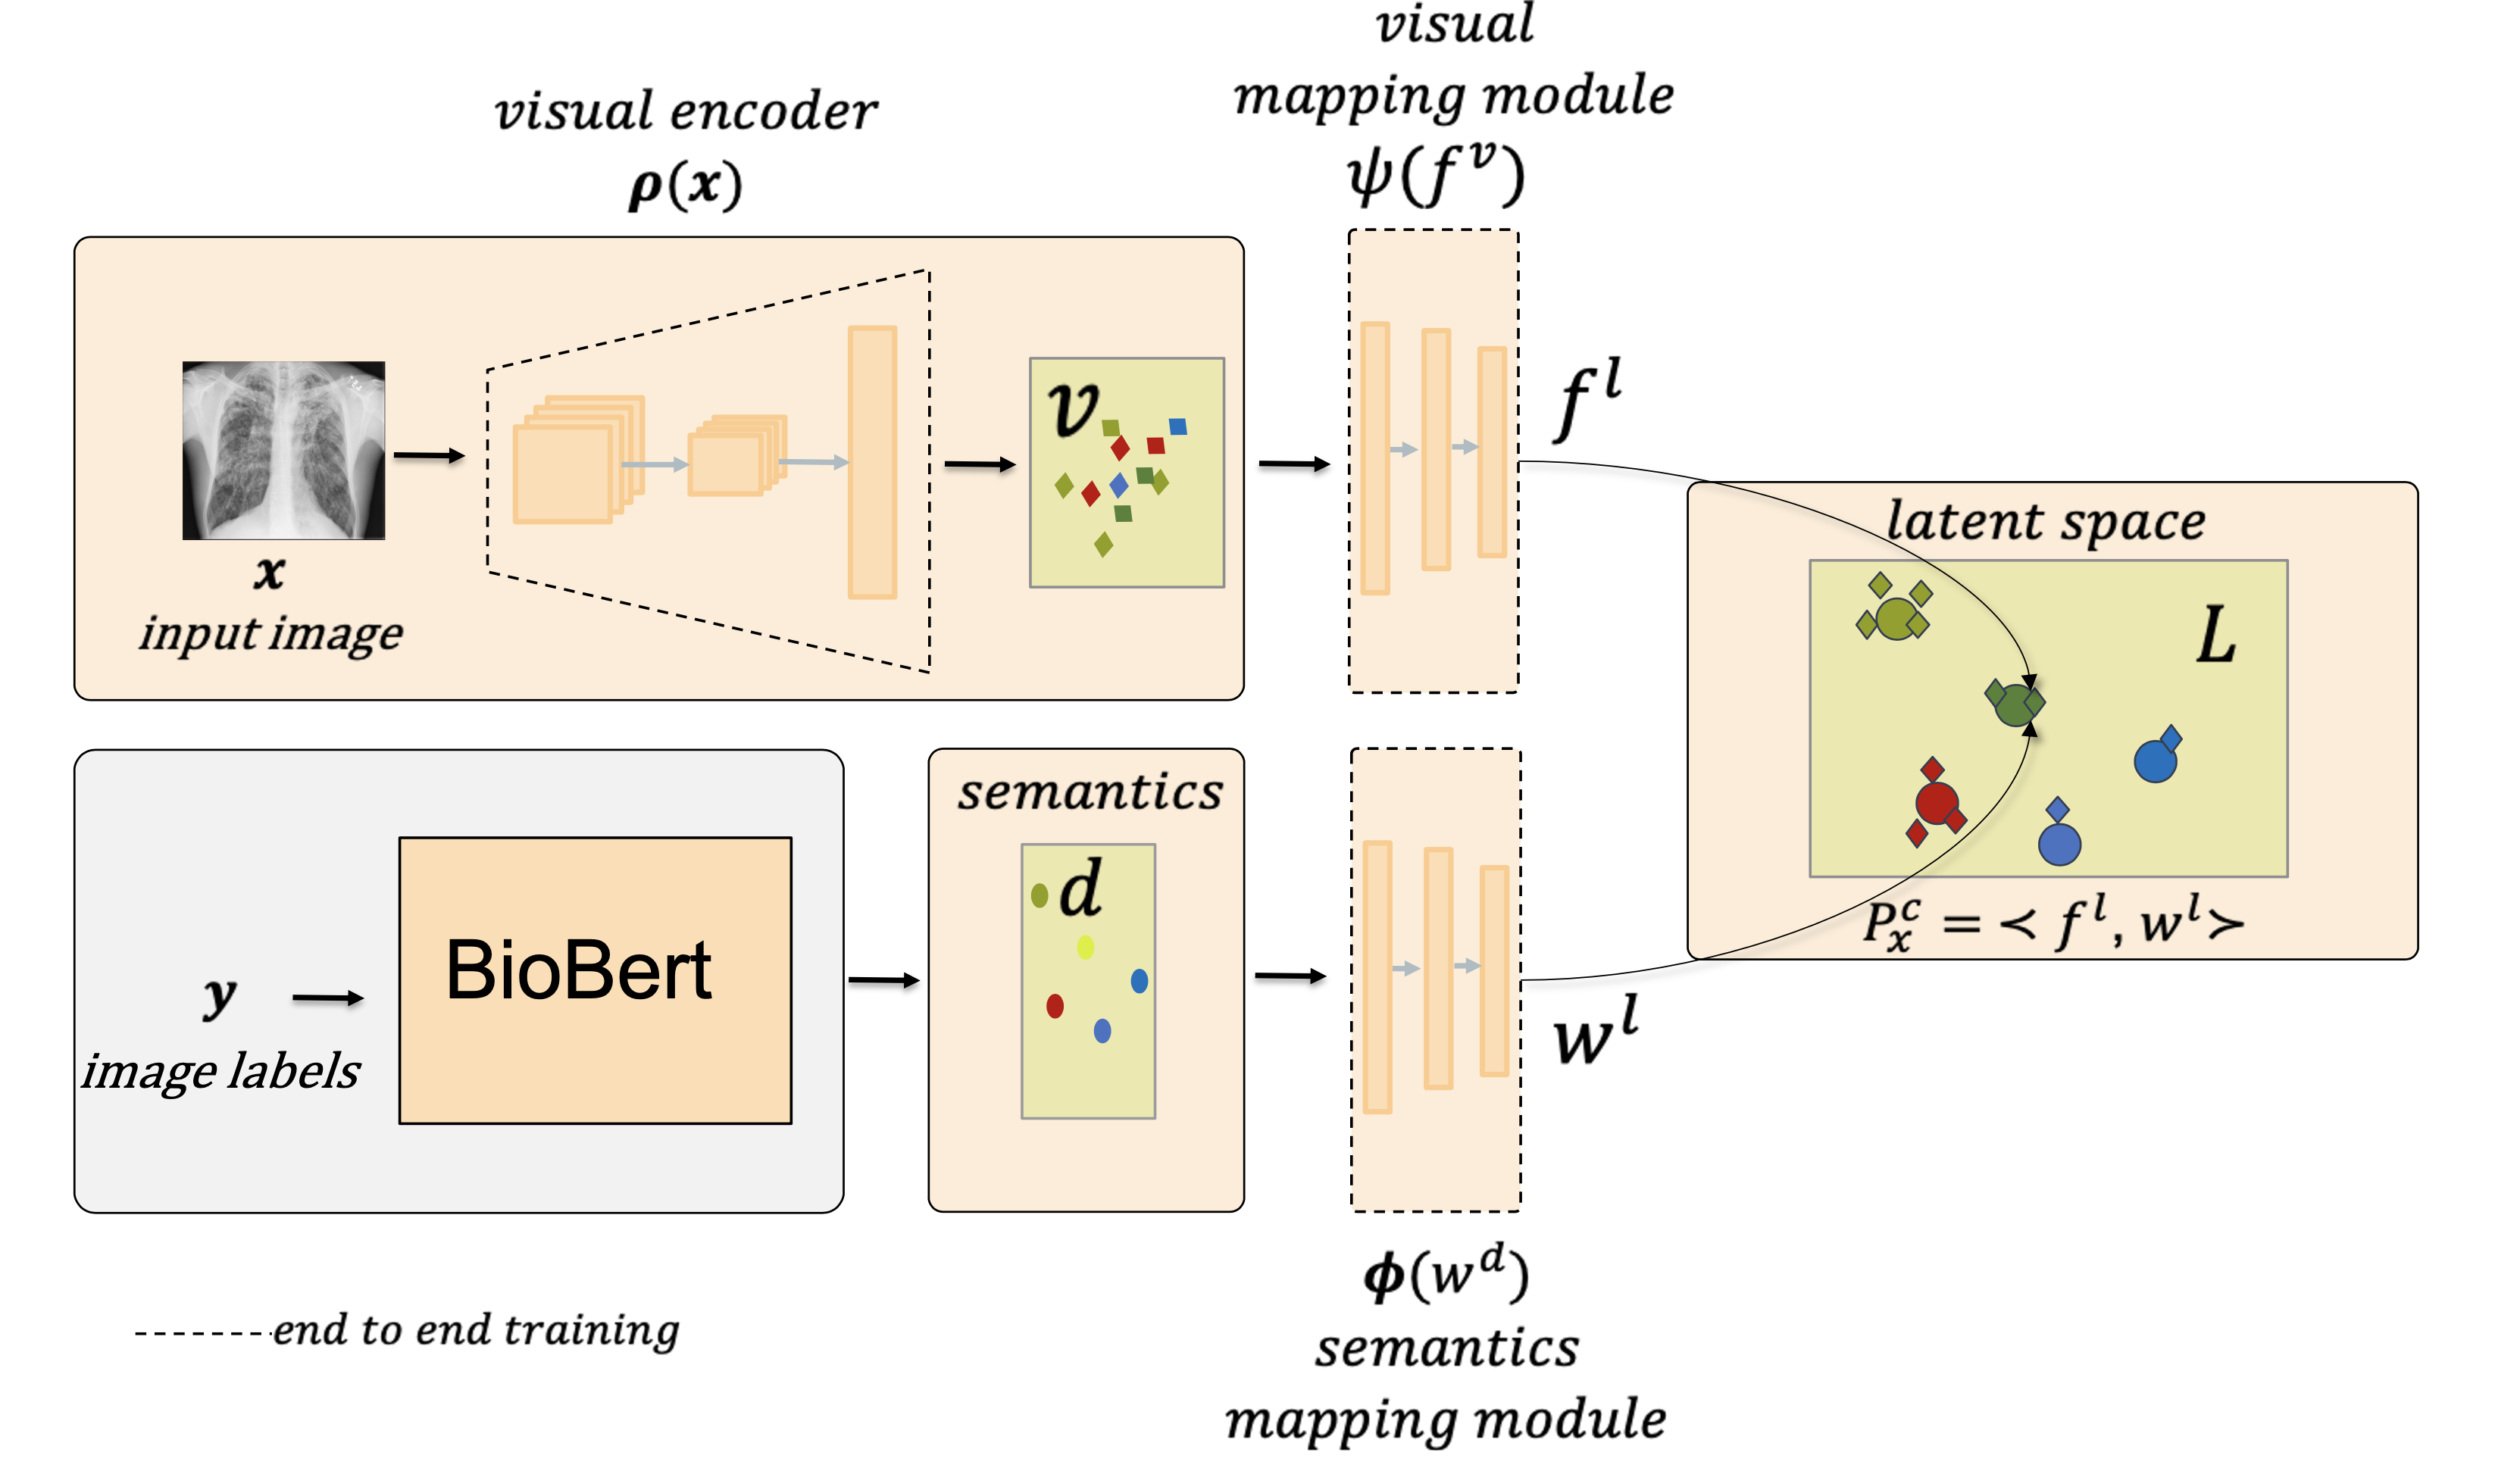
\includegraphics[width=0.9\columnwidth]{model.png}
\caption{CXR-ML-GZSL \cite{hayat2021multilabel}}
\label{fig:model}
\end{figure}

CXR-ML-GZSL is the first use of ML-GZSL to classify diseases from chest X-ray images. It is also unique from other ML-GZSL models in the following three ways.

\begin{itemize}
    \item It can be trained end-to-end, thanks to the trainable visual encoder.
    \item It maps both the semantic and visual embedding spaces into a shared latent embedding space, instead of mapping the visual space onto the semantic space, losing less visual information.
    \item It uses BioBERT, which was trained on a biomedical corpora, resulting semantic embeddings that are tuned for healthcare use cases.
\end{itemize}

The result is better performance when classifying both seen and unseen diseases in chest X-ray images, compared to two state-of-the-art ML-GZSL models: LESA \cite{9157745} and MLZSL \cite{lee2018multilabelzeroshotlearningstructured} (Figure~\ref{fig:results}).

\begin{figure}[h!]
\centering
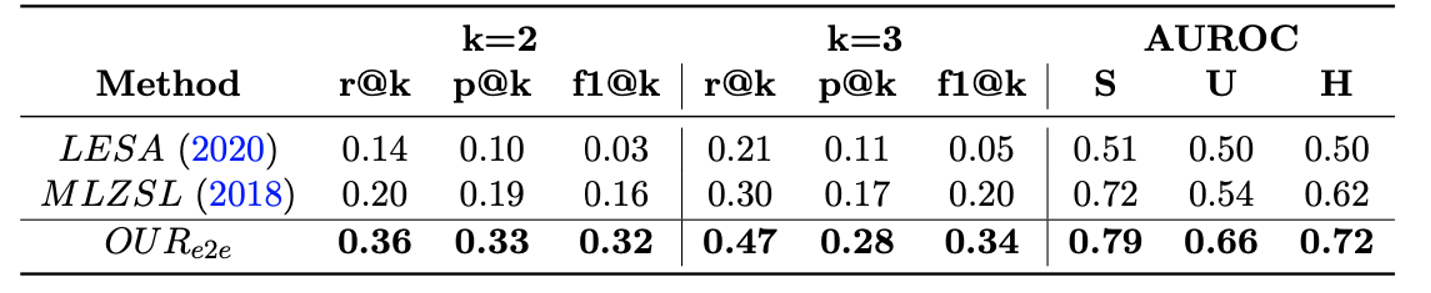
\includegraphics[width=0.9\columnwidth]{results.png}
\caption{Performance of LESA, MLZSL, and CXR-ML-ZSL (``$OUR_{e2e}$") on the ChestX-ray14 database \cite{Wang_2017}. Metrics are precision, recall, f1, and AUROC (split by seen, unseen, and the harmonic mean of the two) \cite{hayat2021multilabel}.}
\label{fig:results}
\end{figure}

\subsection{Scope of Reproducibility}

TBD

\section{Methodology}

\subsection{Environment}

TBD (table of original environment vs reproduction environment)

\subsection{Data}

TBD

\subsection{Model}

TBD (move some of the material from the introduction here?)

\subsection{Training}

TBD

\subsection{Evaluation}

TBD

\section{Results}

TBD

\section{Discussion}

TBD

\section{Contributions}

I completed this project as a team of one. All work, unless otherwise stated, is my own.

\bibliography{report}

\end{document}
